\documentclass{article}
\usepackage[utf8]{inputenc}
\usepackage{graphicx} % Required for inserting images
\usepackage[a4paper, margin=1in]{geometry}
\usepackage[czech]{babel}
\usepackage{setspace}
\usepackage{adjustbox}

\usepackage{amsmath}
\usepackage{commath}
\usepackage{algorithm}
\usepackage{algorithmicx}

\begin{document}

% ÚVODNÍ STRÁNKA
\begin{titlepage}
    \centering
    \Large\textbf{Univerzita Karlova}
    
    \Large{Přírodovědecká fakulta}
    
    \vspace*{2.5cm}
    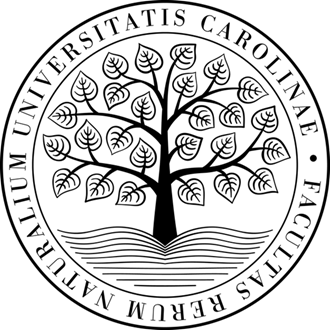
\includegraphics[width=0.55\linewidth]{images/prf.png}
    \vspace*{4cm}
    
    \Large\textbf{ALGORITMY POČÍTAČOVÉ KARTOGRAFIE}
    
    \Large{Generalizace budov}
    
    \vspace*{3cm}
    \large Martina Pavlová, Martin Šíma, Ludmila Vítková

    1 N-GKDPZ
    
    Praha 2024
\end{titlepage}

% ZADÁNÍ
\begin{spacing}{1.5}
\section*{Zadání}

\subsection*{\textbf{Úloha č. 2: Generalizace budov}}

\textit{Vstup: množina budov B = \{$B_i$\}$_{i=0}^n$, budova $B_i = $  \{$P_{i,j}$\}$_{j=1}^m$.}

\noindent\textit{Výstup: $G(B_i)$}


\noindent Ze souboru načtěte vstupní data představovaná lomovými body budov a proveďte generalizaci budov do úrovně detailu LOD0. Pro tyto účely použijte vhodnou datovou sadu, např. ZABAGED, testování proveďte nad třemi datovými sadami (historické centrum města, intravilán – sídliště, intravilán – izolovaná zástavba)

\noindent Pro každou budovu určete její hlavní směry metodami

\begin{itemize}
  \item Minimum Area Enclosing Rectangle
  \item PCA
\end{itemize}
 
\noindent U první metody použijte některý z algoritmů pro konstrukci konvexní obálky. Budovu při generalizaci do úrovně LOD0 nahraďte obdélníkem orientovaným v obou hlavnách směrech, se středem v těžišti budovy, jeho plocha bude stejná jako plocha budovy. Výsledky generalizace vhodně vizualizujte.

\noindent Otestujte a porovnejte efektivitu obou metod s využitím hodnotících kritérií. Pokuste se rozhodnout, pro které tvary budov dávají metody nevhodné výsledky a pro které naopak poskytují vhodnou aproximaci 


\subsection*{\textbf{Hodnocení}}
\vspace{0.3cm}
\begin{adjustbox}{width=1\textwidth}
\begin{tabular}{|l|c|}
\hline
\textbf{Krok}                                                                                  & \textbf{hodnocení} \\ \hline
Generalizace budov metodami Minimum Area Enclosing Rectangle a PCA.                                    &  15b              \\ \hline
\textit{Generalizace budov metodou Longest Edge}                    & \textit{+5b}    \\ \hline
\textit{Generalizace budov metodou Wall Average} & \textit{+8b}    \\ \hline
\textit{Generalizace budov metodou Weighted Bisector}   & \textit{+10b}    \\ \hline
\textit{Implementace další metody konstrukce konvexní obálky} & \textit{+5b} \\ \hline
\textit{Ošetření singulárních případů při generování konvexní obálky}                    & \textit{+2b}    \\ \hline
\textbf{Max celkem:}                                                                                  & \textbf{45b} \\ \hline
\end{tabular}
%\end{center}
\end{adjustbox}

\vspace{1cm}
\noindent Řešeny byly všechny bonusové úlohy.
\newpage

\section{Popis a rozbor problému}
Generalizace budov je proces, při kterém dochází k redukci detailů a zjednodušení geometrických tvarů budov tak, aby byly vhodné pro zobrazování na mapách různých měřítek. Je nezbytným procesem pro vytváření map, jelikož díky ní lze zachovat přehlednost a čitelnost map. Metody kartografické generalizace se dají dělit do několika skupin, kterými jsou například generalizace výběrem, geometrická generalizace, generalizace reklasifikací, generalizace ploch či generalizace atributů.

\subsection{Konvexní obálka}
Pokud definujeme množinu $n$ bodů $S$ v rovině, pak je konvexní obálkou nejmenší konvexní mnohoúhelník $P$, který obsahuje množinu bodů $S$. Zároveň množinu bodů $S$ můžeme označit jako konvexní pouze v~případě, kdy spojnice dvou libovolných prvků leží zcela uvnitř dané množiny bodů. Na obrázku 1 se nachází grafické znázornění konvexní obálky. 

\begin{figure}[h]
    \centering
    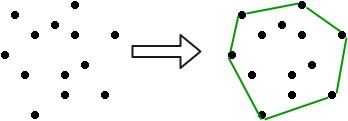
\includegraphics[width=0.7\linewidth]{images/convex.jpg}
    \caption{Konvexní obálka (Sharma 2024a)}
    \label{fig:enter-label}
\end{figure}

Konvexní obálky jsou používány mnoha různými algoritmy, jelikož je díky nim možné s velkou rychlostí najít tzv. bounding box nebo min-max box. Jedná se o objekt, který představuje nejzákladnější generalizaci polygonu a je to takový obdélník, který je kolmý na osy souřadnicového systému a zároveň minimálně ohraničuje daný polygon. Konvexní obálky mohou být dále použity například pro detekci kolizí, k analýze tvarů či statistické analýze.

Existuje více různých způsobů, jak konvexní obálku zkonstruovat. V této práci byly implementovány dva algoritmy, a to Jarvis Scan a Graham Scan. 

\subsubsection{Jarvis Scan }
Jarvis Scan neboli Gift Wrapping Algorithm je jednoduchým, snadno implementovatelným a také jedním z nejvíce používaných algoritmů pro tvorbu konvexní obálky v rovině. Tento algoritmus předpokládá, že se v dané množině bodů $S$ nenachází tři kolineární body. Tento algoritmus funguje tak, že opakovaně hledá největší úhel $\omega$ mezi poslední hranou konvexní obálky a následující hranou. Poslední hrana je tvořena body $p_{j-1}$, $p_j$ a následující hrana je tvořena body $p_j$, $p_{j+1}$. Bod $p_{j+1}$ je hledán pouze mezi body, které ještě nejsou součástí konvexní obálky. Prvním krokem při implementaci tohoto algoritmu je nalezení počátečního bodu (pivot), přičemž tento bod se automaticky stane součástí konvexní obálky. Algoritmus skončí v případě, že se aktuální bod konvexní obálky rovná bodu počátečnímu a dojde tak k vytvoření celé konvexní obálky. Tento algoritmus se nehodí pro velké datasety, jelikož jeho časová složitost je $O(n^2)$. Na obrázku 2 je vidět grafické znázornění průběhu tohoto algoritmu.

\begin{figure}[h]
    \centering
    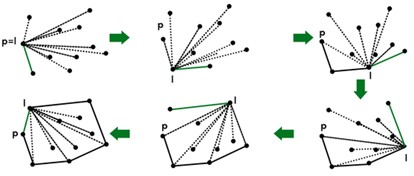
\includegraphics[width=0.75\linewidth]{images/jarvis.jpg}
    \caption{Jarvis Scan (Greyrat 2022)}
    \label{fig:enter-label}
\end{figure}

\subsubsection*{Implementace algoritmu Jarvis Scan}
\begin{algorithm}
    \caption {\textit{Jarvis Scan}}
    \begin{algorithmic}[1]
        \State Inicializuj prázdnou množinu $ch$
        \State Najdi pivota $q$, který má nejmenší y-ovou souřadnici
        \State Najdi pivota $s$, který má nejmenší x-ovou souřadnici
        \State  Inicializuj poslední dva body konvexní obálky $qj$ a $qj_1$
        \State Přidej pivota do konvexní obálky
        \State While True
        \State \indent Inicializuj proměnné $omegaMax$ a $indexMax$
        \State \indent Projdi všechny body polygonu
        \State \indent \indent Pokud bod polygonu není totožný s aktuálním bodem konvexní obálky
        \State \indent \indent \indent Vypočítej úhel $omega$
        \State \indent \indent \indent Pokud je $omega$ větší než $omegaMax$
        \State \indent \indent \indent Aktualizuj úhel $omegaMax$ a $indexMax$
        \State \indent Přidej bod do konvexní obálky $ch$
        \State \indent Pokud je bod pivotem
        \State \indent \indent Skonči
        \State \indent Aktualizuj poslední segment konvexní obálky
        \State  Vrať konvexní obálku
    \end{algorithmic}
\end{algorithm}

\subsubsection{Graham Scan }
Dalším algoritmem, který lze použít pro sestrojení konvexní obálky je Graham Scan, který byl jedním z prvních takových algoritmů. Při aplikaci tohoto algoritmu dochází k využití kritéria pravotočivosti (příp. levotočivosti), kde se posuzuje úhel $\omega_i$. Tento úhel je mezi dvěma úsečkami, které procházejí body $p_{j-1}$, $p_j$ a $p_{j+1}$. Prvním krokem je stejně jako u předchozího algoritmu nalezení počátečního bodu $q$ (pivot). Tento bod se většinou hledá tak, aby jeho y-ová souřadnice byla nejmenší. Vzhledem k tomu, že může existovat více bodů se stejnou y-ovou souřadnicí, vybírá se bod, který z nich má nejmenší x-ovou souřadnici. Dalším krokem je setřídění všech bodů vzestupně na základě jejich hodnoty úhlu $\omega_i$ mezi osou $x$ a spojnicí bodů $q$ a $p_j$. Pokud nastane situace, kdy jsou úhly $\omega_i$ u více bodů stejné, dojde k~seřazení bodů podle jejich euklidovské vzdálenosti od bodu $q$. 

\begin{figure}[h]
    \centering
    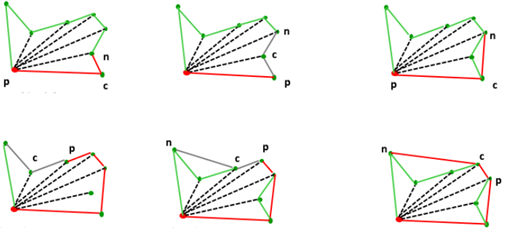
\includegraphics[width=0.75\linewidth]{images/graham.png}
    \caption{Graham Scan (Sharma 2024b)}
    \label{fig:enter-label}
\end{figure}

Spojením všech setříděných bodů se vytvoří nekonvexní mnohoúhelní, který se následně převede na mnohoúhelník konvexní. Tento proces lze vidět na obrázku 3. Jeho časová složitost je $O(n\cdot log(n))$ a lze tedy použít i pro rozsáhlé datasety. 

\subsubsection*{Implementace algoritmu Graham Scan}
\begin{algorithm}
    \caption {\textit{Graham Scan}}
    \begin{algorithmic}[1]
        \State Inicializuj prázdný polygon
        \State Najdi bod $q$, který má nejmenší y-ovou souřadnici
        \State Vytvoř prázdný polygon $tmp$
        \State Projdi každý bod v původním polygonu
        \State \indent	Pokud aktuální bod není stejný jako pivot
        \State \indent	\indent	Přidej ho do $tmp$
        \State Aktualizuj polygon
        \State Seřaď body podle úhlu, který svírají s osou x vzhledem k pivotu
        \State Vytvoř prázdný zásobník $S$
        \State Přidej pivot $q$ do $S$
        \State Přidej první bod ze seznamu $sorted\_points$ do $S$
        \State Urči počet bodů v polygonu $pol$
        \State Inicializuj proměnnou $j$ na hodnotu 2
        \State Projdi všechny seřazené body od druhého bodu
        \State \indent	Přiřaď aktuální bod $pj$ ze seznamu $sorted\_points$
        \State \indent	Pokud bod leží vlevo
        \State \indent	\indent	Přidej ho do $pj$
        \State \indent	\indent	Inkrementuj proměnnou $j$ o 1
        \State \indent	Jinak odstraň poslední bod 
        \State Pro každý bod v $S$
        \State \indent	Přidej bod do konvexní obálky
        \State Vrať $ch$
    \end{algorithmic}
\end{algorithm}


\subsubsection{Singulární případy}
U obou výše zmíněných algoritmů pro tvorbu konvexní obálky se vychází z předpokladu, že počet vrcholů polygonu je větší než 2. Pokud by byl počet bodů menší než 2 nejednalo by se o polygon a nemohlo by tím pádem dojít k vytvoření konvexní obálky. Ve vlastním kódu je tedy podmínka, že polygon nesmí mít méně než 3 body.
Dále je také nutné, aby dvě úsečky, mezi kterými se měří úhel nebyly nulové. Při výpočtu úhlu mezi třemi body ($qj$, $qj1$ a $p$) se, mimo jiné, počítá také velikost daných vektorů ($v$, $u$), které poté figurují ve jmenovateli:
$$\cos\varphi=\frac{v \cdot u}{\norm{v}\norm{u}}$$

Dále každý výpočet úhlu probíhá pouze pro body, které se nerovnají $p_j$. Touto podmínkou je zaručeno, že úhel bude počítán mezi třemi unikátními body, a tudíž vektory mají nenulovou velikost. 


\subsection{Detekce hlavních směrů budov}
Abychom mohli jakoukoliv budovu generalizovat, je potřeba najít její hlavní směry. Tímto dojde k~zachování orientace původního objektu a také návaznosti na ostatní prvky v mapě. Předejde se tím tak například tomu, aby budova přesahovala okolní liniové prvky (silnice, potok). Pro nalezení hlavních směrů budov existuje několik různých algoritmů. V této práci došlo k použití algoritmů Minimum Area Enclosing Rectangle, Principal Component Analysis, Longest Edge, Wall Average a Weighted Bisector. Všechny tyto algoritmy jsou popsány v následujících odstavcích. 

\subsubsection{Minimum Area Enclosing Rectangle}
Minimum Area Enclosing Rectangle (MAER) neboli také Minimum Area Bounding Rectangle funguje na principu nalezení takového obdélníku, jehož plocha je minimální. Grafické znázornění tohoto algoritmu lze vidět na obrázku 4. Na počátku je definována množina $n$ bodů $S$ v rovině. Dále proběhne zpracování této množiny do konvexní obálky a následně je vytvořen obdélník, který opíše množinu $S$. Výsledný obdélník má alespoň jednu stranu kolineární s hranou konvexní obálky.

Tento algoritmus prochází postupně všechny hrany konvexní obálky, přičemž pro každou z nich hledá min-max box, který má hranu rovnoběžnou s aktuální hranou konvexní obálky. Ze všech vzniklých obdélníků se následně vybere ten, jehož plocha je minimální.

Algoritmus řeší problém v čase $O(n\cdot log(n))$ a jeho alternativou je algoritmus \textit{Rotating Calipers}, který má časovou složitost $O(n)$. 

\begin{figure}[h]
    \centering
    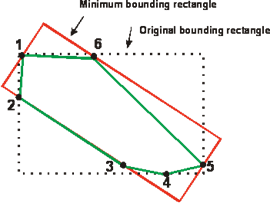
\includegraphics[width=0.5\linewidth]{images/maer.png}
    \caption{Minimum Area Enclosing Rectangle (Scientificlib.com 2024)}
    \label{fig:enter-label}
\end{figure}

\newpage
\subsubsection*{Implementace algoritmu Minimum Area Enclosing Rectangle}
\begin{algorithm}[h]
    \caption {\textit{Minimum Area Enclosing Rectangle}}
    \begin{algorithmic}[1]
        \State Pokud je k dispozici méně než 3 body
        \State \indent Vrať prázdný polygon
        \State Vytvoř konvexní obálku
        \State Inicializuj proměnnou $mmb\_min$ 
        \State Inicializuj proměnnou $area\_min$
        \State Inicializuj proměnnou $sigma\_min$
        \State Učti počet bodů v konvexní obálce
        \State Projdi všechno body konvexní obálky
        \State \indent Vypočítej rozdíl souřadnic mezi aktuálním bodem a následujícím bodem v konvexní obálce
        \State \indent Vypočítej úhel mezi těmito dvěma body
        \State \indent Otoč konvexní obálku o úhel $-sigma$
        \State \indent Vypočítej minimální obdélník
        \State \indent Vypočítej plochu minimálního obdélníku
        \State \indent Pokud je plocha aktuálního obdélníku menší než minimální plocha
        \State \indent \indent Aktualizuj minimální obdélník
        \State \indent \indent Aktualizuj minimální plochu  
        \State \indent \indent Aktualizuj úhel $sigma$	
        \State Otoč minimální obdélník o úhel $sigma\_min$
        \State  Uprav velikost obdélníku 
        \State Vrať $mmb\_res$
    \end{algorithmic}
\end{algorithm}

\subsubsection{Principal Component Analysis (PCA)}
Algoritmus Principal Component Analysis funguje na principu, nalezení hlavních směrů pomocí kovarianční matice $C$ a následným singulárním rozkladem. Kovarianční matici vypadá následovně:

$$C\ =\ \begin{bmatrix}
        C(A, A)&C(A, B)\\
        C(B, A)&C(B,B)
        \end{bmatrix}$$

Pro singulární rozklad (SVD) platí $C = U\mathrm{\Sigma}V^T$.

$$\begin{bmatrix}
c_{11}&c_{12}\\c_{21}&c_{22}
\end{bmatrix}
= 
\begin{bmatrix}
u_{11}&u_{12}\\u_{21}&u_{22}
\end{bmatrix}
\begin{bmatrix}
\sigma_1&0\\0&\sigma_2
\end{bmatrix}
\begin{bmatrix}
(v_{11}&v_{12}\\v_{2}1&v_{22})
\end{bmatrix}^T$$


Úhel, o který budeme polygon následně otáčet se vypočítá jako:

$$\sigma = atan2(v_{12},v_{11}) $$

Tato metoda generalizace budov je snadno zobecnitelná i do vyšších dimenzí. Pro pravidelné objekty, jako jsou například čtverce či kruhy, má tento algoritmus nízkou efektivitu, jelikož vrcholy tím pádem leží na kružnici a neexistuje tak dominantní směr. Jedná se o poměrně citlivou metodu. 

\newpage
\subsubsection*{Implementace algoritmu PCA}
\begin{algorithm}[h]
    \caption {\textit{Principal Component Analysis }}
    \begin{algorithmic}[1]
        \State Pokud je k dispozici méně než 3 body
        \State \indent Vrať prázdný polygon
        \State Vytvoř list souřadnic 
        \State Projdi všechny body polygonu
        \State \indent Přidej souřadnice aktuálního bodu do seznamu
        \State Vytvoř numpy pole
        \State Vypočítej kovarianční matici souřadnic bodů polygonu
        \State Proveď singulární rozklad kovarianční matice
        \State Vypočítej úhel pro převrácen polygonu
        \State Otoč polygon o úhel $-sigma$
        \State Vytvoř minimální obdélník pro daný polygon
        \State  Otoč minimální obdélník o úhel $sigma$
        \State Uprav velikost obdélníku 
        \State Vrať $er\_r$
    \end{algorithmic}
\end{algorithm}

\subsubsection{Longest Edge}
Algoritmus Longest Edge je jednoduchou metodou generalizace budov, která funguje na principu, kdy je hlavní směr budovy přestavován nejdelší stranou dané budovy. Druhý hlavní je směr je na něj pak kolmý. Výsledný polygon je tedy natočený podél nejdelší strany budovy a zároveň je jeho delší strana rovnoběžná s touto nejdelší stranou budovy. Tento algoritmus nedosahuje příliš dobrých výsledků, jelikož nejdelší strana nemusí nutně reprezentovat hlavní směr budovy.

\subsubsection*{Implementace algoritmu Longest Edge}
\begin{algorithm}[h]
    \caption {\textit{Longest Edge}}
    \begin{algorithmic}[1]
        \State Urči počet bodů v polygonu
        \State Inicializuj proměnnou $longest\_edge$
        \State Inicializuj proměnnou $angle$
        \State Projdi všechny hrany polygonu
        \State \indent Vypočítej délku aktuální hrany
        \State \indent Pokud je $edge\_length$ větší než $longest\_edge$
        \State \indent \indent Aktualizuj proměnnou $longest\_edge$
        \State \indent \indent Vypočítej sklon hrany
        \State Otoč polygon o úhel $-sigma$
        \State Vytvoř minimální obdélník pro daný polygon
        \State Otoč minimální obdélník o úhel $sigma$
        \State Uprav velikost obdélníku 
        \State Vrať $er\_r$
    \end{algorithmic}
\end{algorithm}

\newpage
\subsubsection{Wall Average}
Algoritmus Wall Average patří k těm komplexnějším. Je založen na principu, kdy je pro každou hranu v~daném polygonu spočítán zaokrouhlený podíl $k_i$: 

$$k_i\ =\ \left\lfloor\frac{\Delta\sigma_i}{\frac{\pi}{2}}\right\rfloor$$

Proměnná $\Delta\sigma_i$ značí rozdíl úhlů $\sigma_i$ a $\sigma'$, kde $\sigma_i$ je směrnice aktuálně zpracované hrany a $\sigma'$ je náhodně zvolená směrnice jedné z hran daného polygonu. Tento rozdíl vypadá tedy následovně:

$$\Delta\sigma_i = \sigma_i - \sigma'$$

Po vypočtení $k_i$ dojde k vypočítání zbytků $r_i$ a odchylky od $0\pm\ k\pi$, respektive $\frac{\pi}{2}\pm\ k\pi$:

$$r_i = \Delta\sigma_i - k_i\frac{\pi}{2}$$

Hlavní směr natočení budovy se následně vypočítá pomocí vztahu:

$$\sigma = \sigma' + \sum_{i = 1}^{n}\frac{r_i\cdot s_i}{s_i}$$

Proměnná $s_i$ značí délku hrany $i$.

\subsubsection*{Implementace algoritmu Wall Average}

\begin{algorithm}[h]
    \caption {\textit{Wall Average}}
    \begin{algorithmic}[1]
        \State Urči počet bodů v polygonu
        \State Vypočítej rozdíl souřadnic mezi prvním a druhým bodem polygonu
        \State Vypočítej směr hrany
        \State Inicializuj proměnnou $av\_r$ 
        \State Projdi všechny hrany polygonu
        \State \indent Vypočítej rozdíl souřadnic mezi aktuálním a následujícím bodem polygonu
        \State \indent Vypočítej směr aktuální hrany polygonu
        \State \indent Vypočítej rozdíl směru mezi aktuální hranou a první hranou
        \State \indent Pokud je $dir\_dif$ větší než 0
        \State \indent \indent Přičti $2\pi$
        \State \indent Vypočítej počet čtvrtin otočení
        \State \indent Vypočítej zbytek po odečtení počtu čtvrtin
        \State \indent Aktualizuj průměrný zbytek 
        \State Vypočítej průměrný zbytek
        \State Vypočítej průměrný úhel rotace
        \State Otoč polygon o úhel $-sigma\_av$
        \State Vytvoř minimální obdélník pro daný polygon
        \State  Otoč minimální obdélník o úhel $sigma\_av$
        \State Uprav velikost obdélníku 
        \State Vrať $er\_r$
    \end{algorithmic}
\end{algorithm}


\subsubsection{Weighted Bisector}
Algoritmus Weighted Bisector používá pro detekci hlavních směrů dvě nejdelší úhlopříčky, které se v~daném polygonu nachází. Jedná se o úhlopříčky, které neprotínají ani jednu z hran polygonu. Z bodů $P_1 = [x_1,\ y_1]$ a $P_2 = [x_2,\ y_2]$ se vytvoří úsečka $P_1P_2$ a z bodů $P_3 = [x_3,\ y_3]$ a $P_4 = [x_4,\ y_4]$ vznikne úsečka $P_3P_4$. Pro tyto body se následně provede čtyřikrát analýza koncového bodu úsečky vzhledem ke druhé úsečce, aby se zjistilo, zda úsečka prochází či neprochází hranou polygonu. Dochází k výpočtu determinantu: 

$$t_1 = \begin{vmatrix} x_2 - x_1 & y_2 - y_1 \\ x_4 - x_1 & y_4 - y_1  \end{vmatrix} \ \ \ \
t_2 = \begin{vmatrix} x_2 - x_1 & y_2 - y_1 \\ x_3 - x_1 & y_3 - y_1  \end{vmatrix}$$

$$t_3 = \begin{vmatrix} x_4 - x_3 & y_4 - y_3 \\ x_1 - x_3 & y_1 - y_3  \end{vmatrix} \ \ \ \
t_4 = \begin{vmatrix} x_4 - x_3 & y_4 - y_3 \\ x_2 - x_3 & y_2 - y_3 \end{vmatrix}$$

Průsečík neexistuje buď pokud mají $t_1$ a $t_2$ stejné znaménko anebo pokud $t_3$ a $t_4$ mají stejné znaménko. Znamená to totiž, že se oba body nacházejí ve stejné polorovině vůči druhé úsečce. Úsečka je tím pádem úhlopříčkou, přičemž následně dojde k výběru dvou nejdelších úhlopříček a je pro ně spočítána jejich směrnice. Hlavní směr budovy $\sigma$ je poté určen jako vážený průměr směrnic nejdelších úhlopříček, kde jsou váhami délky uhlopříček. Vzorec pro tento výpočet vypadá tedy takto:  

$$\sigma\ =\ \frac{s_1\sigma_1\ +\ s_2\sigma_2}{s_1\ +\ s_2}$$

\subsubsection*{Implementace algoritmu Weighted Bisector}

\begin{algorithm}[h]
    \caption {\textit{Weighted Bisector}}
    \begin{algorithmic}[1]
        \State Pokud je k dispozici méně než 3 body
        \State \indent Vrať prázdný polygon
        \State Najdi dvě nejdelší diagonály polygonu
        \State Vypočítej sklon první a druhé diagonály
        \State Vypočítej vážený průměr úhlů diagonál $sigma$ 
        \State Otoč polygon o úhel $-sigma$
        \State Vytvoř minimální obdélník pro daný polygon
        \State Otoč minimální obdélník o úhel $sigma$
        \State Uprav velikost obdélníku 
        \State Vrať $er\_res$
    \end{algorithmic}
\end{algorithm}

\newpage
\subsection{Hodnocení efektivity detekce hlavních směrů}
Pro porovnání jednotlivých algoritmů na generalizaci budov došlo k definování hodnocení efektivity detekce hlavních směrů. Toto hodnocení se zpravidla provádí na jednotlivých objektech a jeho předpokladem je, že budovy jsou pravoúhlé. Základem je určení nejdelší strany generalizované budovy. Byla vypočítána střední hodnota úhlových odchylek jednotlivých segmentů, pro kterou platí vztah: 

$$\Delta\sigma_1\ =\ \frac{\pi}{2n} \sum_{i = 1}^{n} [r_i - r]$$

kde

$$r_i\ =\ (k_i- \left\lfloor k_i\right\rfloor)\frac{\pi}{2},\ \ \ \ \ \ k_i = \frac{{2\sigma}_i}{\pi}$$

Druhým výpočtem je střední hodnota čtverců úhlových odchylek jednotlivých segmentů:

$$\Delta\sigma_2\ =\ \frac{\pi}{2n}\sqrt{\sum_{i = 1}^{n}{({r_i - r)}^2}}$$

\section{Struktura programu}
Program se skládá ze sedmi souborů, kterými jsou \textit{Data}, \textit{Images}, \textit{Algorithms}, \textit{Building}, \textit{Draw}, \textit{Load} a~\textit{MainForm}. 

Ve složce \textit{Data} se nacházejí vstupná data, která se skládají z pěti různých souborů. Prvním z nich je soubor budov, které se nacházejí v centru města a jsou tedy velmi blízko sebe. Pro tento dataset bylo vybráno Staré Město v Praze. Druhým datasetem jsou budovy, které se nacházejí na sídlišti a mají tedy většinou pravidelný tvar. V tomto případě se jedná o sídliště Opatov. Třetí dataset obsahuje vilovou oblast Mydlářka, kde stojí budovy samostatně dá od sebe. Další dataset zobrazuje oblast Vinohrad a~poslední dataset s názvem \textit{Test} obsahuje pouze jeden polygon. Všechny tyto datasety jsou ve formátu JSON. Ve vstupních datech je klíč POLYGONS, který obsahuje seznam budov, kde je každá budova reprezentována seznamem bodů ve formátu [x, y].  Každá souřadnice je zadána jako desetinné číslo s~devíti desetinnými místy. Jelikož se jedná o uzavřené polygony, je první a poslední bod u každé budovy totožný. 

Ve složce \textit{Images} se nachází celkem 15 ikon, které slouží k vytvoření aplikace. Těmito ikonami jsou \textit{Jarvis\_scan.png}, \textit{Graham\_scan.png}, \textit{Validate.png}, \textit{about.png}, \textit{ch.png}, \textit{clear.png}, \textit{clear\_ch.png}, \textit{clear\_er.png}, \textit{exit.png}, \textit{longestedge.png}, \textit{maer.png}, \textit{open\_file.png}, \textit{pca.png}, \textit{wa.png}, \textit{weightedbisector.png}. 

V \textit{Algorithms.py} je definována třída \textit{Algorithms}, která obsahuje skoro dvacet metod. Metoda \textit{errorWindow} slouží k zobrazení informačních, varovných a chybových zpráv pomocí dialogového okna. Pomocí \textit{analyzePointLinePosition} dochází k určení polohy bodu $p$ vzhledem k přímce určené body $p_1$ a $p_2$. Pokud se bod nachází vlevo, je vrácena hodnota 1. V jiném případě je vrácena hodnota 0. Další metodou je \textit{getTwoLineAngle}, která vypočítá pomocí skalárního součinu úhel mezi dvěma liniemi definovanými čtyřmi body. Pro vytvoření konvexní obálky lze použít metodu \textit{jarvisScan} nebo \textit{grahamScan}. Při použití metody implementující Jarvis Scan dojde k nalezení počátečního bodu a následně k vytvoření konvexní obálky na základě maximálního úhlu. Při použití metody Graham Scan dojde také k nalezení počátečního bodu, následně k seřazení bodů a z nich se vytvoří konvexní obálka.  Pomocí metody \textit{mmb} dochází k vytvoření min-max boxu, který obsahuje všechny body vstupního seznamu. Metoda \textit{rotate} slouží k rotaci polygonu o úhel $sig$, metoda \textit{getArea} slouží k výpočtu plochy polygonu a metoda \textit{l2} vypočítá Eukleidovskou vzdálenost mezi dvěma body. V rámci \textit{searchDiagonals} dochází k hledání nejdelších úhlopříček daného polygonu, pomocí \textit{weightedMean} dochází k výpočtu váženého průměru dvou hodnot a \textit{slope} slouží k~výpočtu sklonu úhlopříčky, která je určena dvěma body. Metoda \textit{resizeRectangle} slouží k přizpůsobení velikosti polygonu tak, aby se vešel do oblasti původní budovy. Dalších pět metod slouží k samotné generalizaci budov v závislosti na zvoleném algoritmu. Těmito metodami jsou \textit{createMBR}, \textit{createERPCA}, \textit{longestEdge}, \textit{wallAverage} a \textit{weightedBisector}. Poslední metodou je \textit{validation}, ve které dochází k hodnocení efektivity detekce hlavních směrů. 

V \textit{Building.py} je definována třída \textit{Building}, která slouží k reprezentaci budovy. Dochází k určení počtu vrcholů v polygonu či k přidání vrcholu do polygonu. Slouží k nastavení zjednodušené verze budovy. 

V \textit{draw.py} se nachází třída \textit{Draw}, ve které je definovaných celkem šest různých metod. Metoda \textit{getBuildigns} vrací seznam budov uložených v proměnné \textit{buildings}. Metoda \textit{getJarvis} slouží k přepínání použití algoritmu Jarvis Scan pro vytvoření konvexní obálky. \textit{clearData} slouží ke smazání dat v proměnné \textit{buildings} a \textit{clearmbr} slouží ke smazání polygonů generalizovaných budov. Metoda \textit{mousePressEvent} je zavolána při stisknutí tlačítka myši, přičemž získává souřadnice a přidává nový bod budovy. Poslední metodou je \textit{paintEvent}, která je volána v případě, kdy je potřeba překreslit plátno. Pro každou budovu se vykreslí původní polygon (černý obrys, žlutá výplň) a její zjednodušená verze (červený obrys). 

V \textit{Load.py} dochází k definování \textit{load\_buildings} a \textit{transformBuildings}. Funkce \textit{load\_buildings} slouží k~načtení dat budov ze souboru formátu JSON. Pro každý polygon se projdou všechny body a spočítají se minimální a maximální hodnoty x a y, aby bylo možné určit velikost oblasti, ve které se budovy nacházejí. Pokud při načítání dat dojde k nějaké chybě, objeví se odpovídající chybová hláška. Po načtení dat a určení rozměrů oblasti, ve které se budovy nacházejí, se spočítají posuny $dx$ a $dy$, které umožňují umístit budovy do středu zobrazovací oblasti, a měřítko \textit{scale}, které určuje, jak moc se budovy musí zmenšit/zvětšit, aby se vešly do zobrazovací oblasti. Nakonec se provede transformace souřadnic všech polygonů budov podle vypočtených hodnot měřítka a posunů pomocí funkce \textit{transformBuildings}.

V \textit{MainForm.py} je definována třída \textit{Ui\_MainWindow}, ve které je následně definováno několik metod. Metody \textit{setupUI} a \textit{retranslateUI} byly vygenerovány v prostředí Qt. Nově implementovanými byly metody \textit{openClick}, \textit{mbrClick}, \textit{pcaClick}, \textit{clearClick}, \textit{clearAllClick}, \textit{jarvisScan}, \textit{grahamScan}, \textit{longestEdge}, \textit{wallAverage}, \textit{weightedBisector} a \textit{validation}. Zavolání metody \textit{openClick} proběhne při kliknutí na možnost \textit{Open} v menu. Dochází k otevření dialogového okna pro výběr souboru typu JSON a po výběru souboru dojde pomocí funkce \textit{load\_buildings} k načtení polygonů budov, které jsou následně vykresleny. Metoda \textit{mbrClick} přijímá seznam budov a pro každou z nich vytvoří její ohraničující obdélník pomocí algoritmu Minimum Area Enclosing Rectangle. Metody \textit{pcaClick}, \textit{longestEdge}, \textit{wallAverage} a \textit{weightedBisecto}r fungují stejně jako předchozí metoda, avšak pro algoritmy Principal Component Analysis, Longest Edge, Wall Average a Weighted Bisector. Dalšími dvěma metodami jsou \textit{clearClick} a \textit{clearAllClick}. Pomocí \textit{clearClick} dojde k vymazání všech minimálních ohraničujících obdélníků a po kliknutí na \textit{clearAllClick} dojde ke smazání všech dat. Obě tyto metody nakonec překreslí plátno. Metody \textit{jarvisScan} a \textit{grahamScan} slouží k vytvoření konvexní obálky na základě zvoleného algoritmu. Poslední metodou je \textit{validation}, která provedení hodnocení efektivity detekce hlavních směrů. Výsledek se zobrazí v dialogovém okně. 

\section{Výsledky}
V rámci této úlohy došlo k vytvoření uživatelského rozhraní s využitím frameworku QT, ve kterém je demonstrována funkčnost algoritmů Jarvis Scan a Graham Scan pro tvorbu konvexní obálky a algoritmů Minimum Area Enclosing Rectangle, Principal Component Analysis, Longest Edge, Wall Average a~Weighted Bisector pro generalizaci polygonů budov. Toto grafické rozhraní aplikace vytvořené v prostředí Qt Designer lze vidět na obrázku 5 a dále bylo upravováno v prostředí programovacího jazyka Python. Po spuštění aplikace může uživatel otevřít soubor obsahující polygony budov. 

\begin{figure}[h]
    \centering
    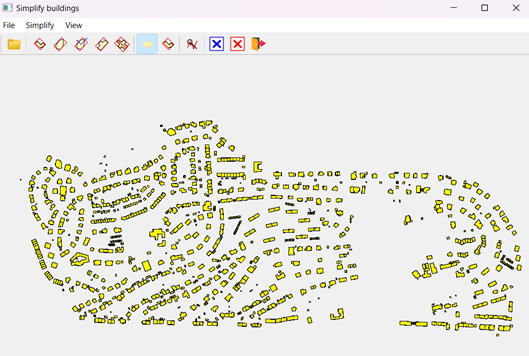
\includegraphics[width=0.6\linewidth]{images/rozhrani.png}
    \caption{Grafické rozhraní aplikace po načtení souboru s polygony budov}
    \label{fig:enter-label}
\end{figure}

V rámci tohoto rozhraní lze zvolit, kterou metodou proběhne tvorba konvexní obálky i samotná generalizace budov. Po zvolení těchto parametrů proběhne analýza dat a dojde k vykreslení generalizovaných polygonů budov červeným obrysem, zatímco původní data mají žlutou výplň a černý obrys. Jak takový výsledek může vypadat lze vidět na obrázku 6.

\begin{figure}[h]
    \centering
    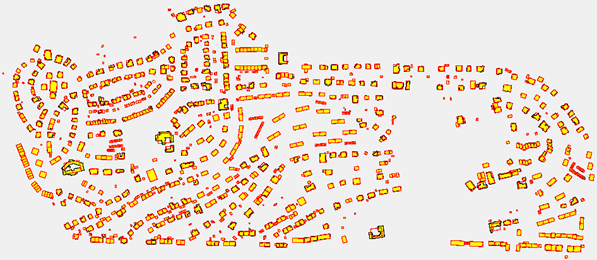
\includegraphics[width=0.6\linewidth]{images/vysledek.png}
    \caption{Ukázka možného výsledku}
    \label{fig:enter-label}
\end{figure}

\newpage
Prvním analyzovaným datasetem bylo Staré Město v Praze. Jedná se o budovy v centru města, které jsou blízko u sebe a mají nepravidelné tvary. Výřez tohoto datasetu lze vidět na obrázku 7. Na obrázcích 8 až 12 jsou vidět výsledky jednotlivých algoritmů pro generalizaci polygonů budov. Při pohledu na tyto obrázky lze vidět, že nejhorší výsledek měl algoritmus Weighted Bisector, zatímco dobrý výsledek měly algoritmy Minimum Area Enclosing Rectangle a Wall Average.

\begin{figure}[htbp]
  \centering
  \begin{minipage}[b]{0.37\textwidth}
    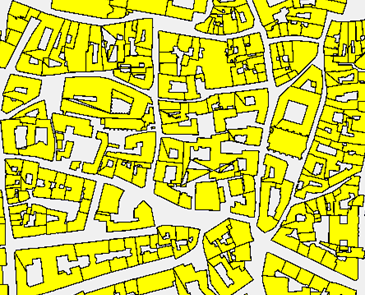
\includegraphics[width=\textwidth]{images/SM_orig.png}
    \caption{Staré Město – původní budovy}
  \end{minipage}
  \hfill
  \begin{minipage}[b]{0.37\textwidth}
    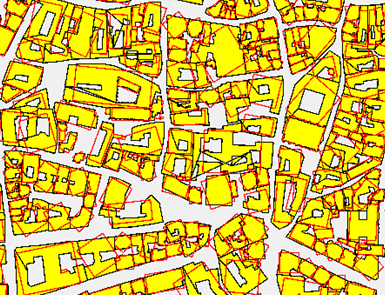
\includegraphics[width=\textwidth]{images/SM_pca.png}
    \caption{Staré Město – výsledek PCA}
  \end{minipage}
\end{figure}

\begin{figure}[htbp]
  \centering
  \begin{minipage}[b]{0.37\textwidth}
    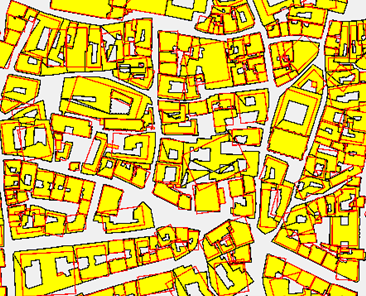
\includegraphics[width=\textwidth]{images/SM_le.png}
    \caption{Staré Město – výsledek LE}
  \end{minipage}
  \hfill
  \begin{minipage}[b]{0.37\textwidth}
    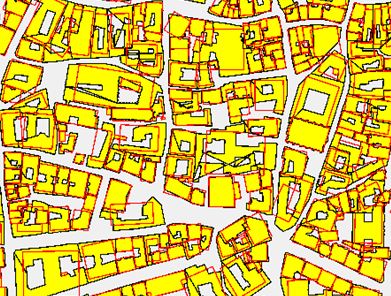
\includegraphics[width=\textwidth]{images/SM_wa.png}
    \caption{Staré Město – výsledek WA}
  \end{minipage}
\end{figure}

\begin{figure}[htbp]
  \centering
  \begin{minipage}[b]{0.37\textwidth}
    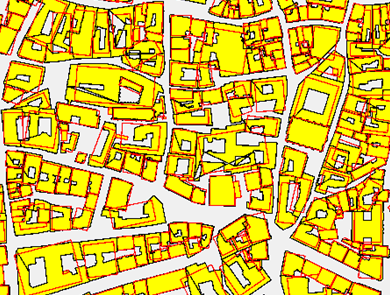
\includegraphics[width=\textwidth]{images/SM_maer.png}
    \caption{Staré Město – výsledek MAER}
  \end{minipage}
  \hfill
  \begin{minipage}[b]{0.37\textwidth}
    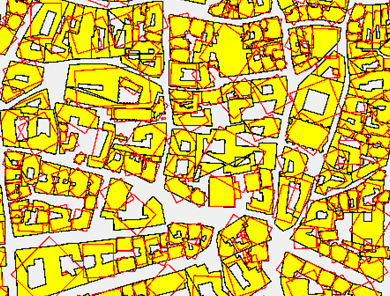
\includegraphics[width=\textwidth]{images/SM_wb.png}
    \caption{Staré Město – výsledek WB}
  \end{minipage}
\end{figure}

\newpage
Druhým analyzovaným datasetem bylo sídliště Opatov v Praze. Jedná se o budovy, které mají pravidelný tvar a jsou uspořádané do bloků. Výřez tohoto datasetu lze vidět na obrázku 13. Na obrázcích 14 až 18 jsou vidět výsledky jednotlivých algoritmů pro generalizaci polygonů budov.  Při pohledu na tyto obrázky lze vidět, že nejhorší výsledek měl opět algoritmus Weighted Bisector, zatímco podobně dobrý výsledky měly algoritmy Longest Edge, Minimum Area Enclosing Rectangle a Wall Average.

\begin{figure}[htbp]
  \centering
  \begin{minipage}[b]{0.43\textwidth}
    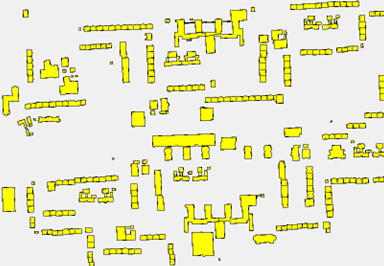
\includegraphics[width=\textwidth]{images/Opatov_orig.png}
    \caption{Opatov – původní budovy}
  \end{minipage}
  \hfill
  \begin{minipage}[b]{0.43\textwidth}
    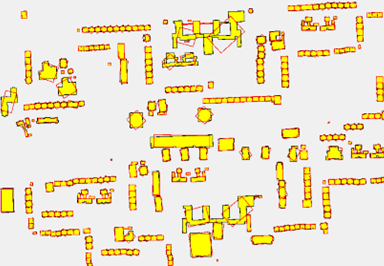
\includegraphics[width=\textwidth]{images/Opatov_pca.png}
    \caption{Opatov – výsledek PCA}
  \end{minipage}
\end{figure}

\begin{figure}[htbp]
  \centering
  \begin{minipage}[b]{0.43\textwidth}
    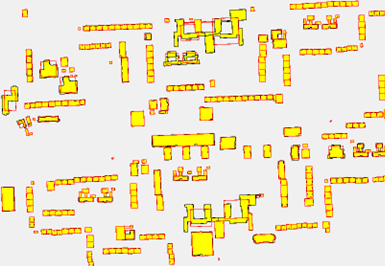
\includegraphics[width=\textwidth]{images/Opatov_le.png}
    \caption{Opatov – výsledek LE}
  \end{minipage}
  \hfill
  \begin{minipage}[b]{0.43\textwidth}
    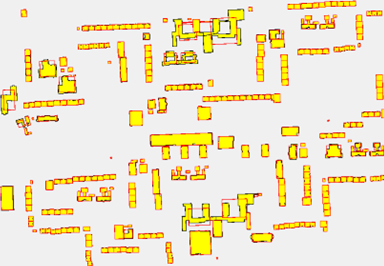
\includegraphics[width=\textwidth]{images/Opatov_wa.png}
    \caption{Opatov – výsledek WA}
  \end{minipage}
\end{figure}

\begin{figure}[htbp]
  \centering
  \begin{minipage}[b]{0.43\textwidth}
    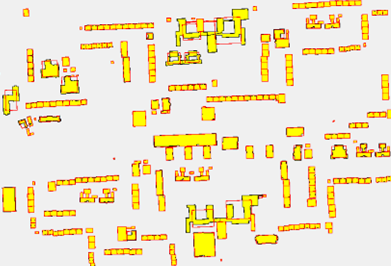
\includegraphics[width=\textwidth]{images/Opatov_maer.png}
    \caption{Opatov – výsledek MAER}
  \end{minipage}
  \hfill
  \begin{minipage}[b]{0.43\textwidth}
    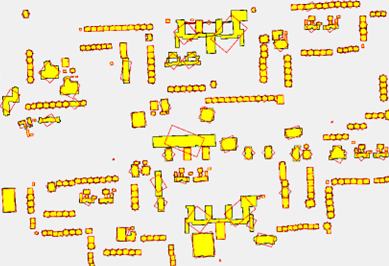
\includegraphics[width=\textwidth]{images/Opatov_wb.png}
    \caption{Opatov – výsledek WB}
  \end{minipage}
\end{figure}

\newpage
Posledním analyzovaným datasetem byla Mydlářka v Praze. Jedná se o vilovou oblast, kde jsou samostatně stojící budovy umístěny daleko od sebe. Výřez tohoto datasetu lze vidět na obrázku 19. Na obrázcích 20 až 24 jsou vidět výsledky jednotlivých algoritmů pro generalizaci polygonů budov. Na první pohled z těchto obrázků nelze říct, který z algoritmů byl nejlepší či nejhorší.

\begin{figure}[htbp]
  \centering
  \begin{minipage}[b]{0.47\textwidth}
    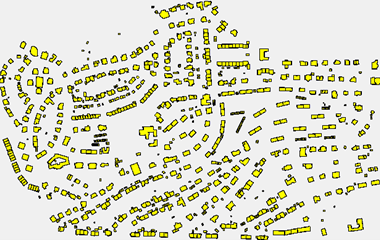
\includegraphics[width=\textwidth]{images/Mydl_orig.png}
    \caption{Mydlářka – původní budovy}
  \end{minipage}
  \hfill
  \begin{minipage}[b]{0.47\textwidth}
    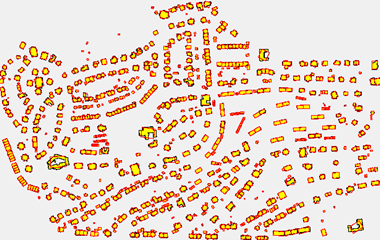
\includegraphics[width=\textwidth]{images/Mydl_pca.png}
    \caption{Mydlářka – výsledek PCA}
  \end{minipage}
\end{figure}

\begin{figure}[htbp]
  \centering
  \begin{minipage}[b]{0.47\textwidth}
    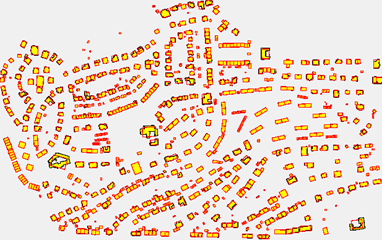
\includegraphics[width=\textwidth]{images/Mydl_le.png}
    \caption{Mydlářka – výsledek LE}
  \end{minipage}
  \hfill
  \begin{minipage}[b]{0.47\textwidth}
    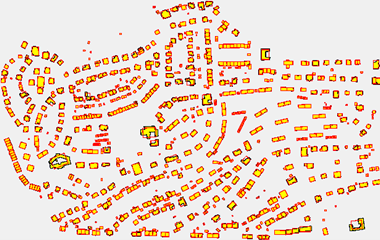
\includegraphics[width=\textwidth]{images/Mydl_wa.png}
    \caption{Mydlářka – výsledek WA}
  \end{minipage}
\end{figure}

\begin{figure}[htbp]
  \centering
  \begin{minipage}[b]{0.47\textwidth}
    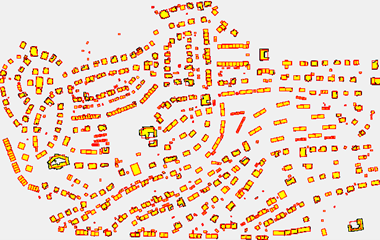
\includegraphics[width=\textwidth]{images/Mydl_maer.png}
    \caption{Mydlářka – výsledek MAER}
  \end{minipage}
  \hfill
  \begin{minipage}[b]{0.47\textwidth}
    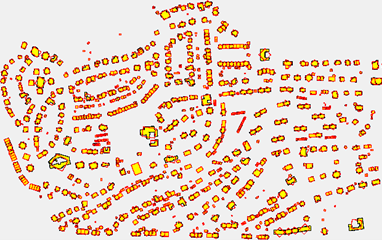
\includegraphics[width=\textwidth]{images/Mydl_wb.png}
    \caption{Mydlářka – výsledek WB}
  \end{minipage}
\end{figure}


\newpage
\subsection{Hodnocení efektivity}
Prvním výpočtem byla střední hodnota úhlových odchylek jednotlivých segmentů. Výsledky jednotlivých algoritmů lze vidět v tabulce 1, kde je uvedeno kolik procent budov mělo hodnotu menší než 10 °. Na posledním řádku této tabulky je vypočítána úspěšnost jednotlivých datasetů.  Nejlepší výsledky měl dataset Mydlářka, kde jsou samostatně stojící domy pravidelného tvaru, které se nacházejí daleko od sebe. Největší úspěšnost měl algoritmus Minimum Area Enclosing Rectangle, který měl více než 73~\% úspěšnost. Algoritmy Longest Edge a Wall Average měli přibližně jen o jedno procento horší úspěšnost. Nejhůře dopadl algoritmus Weighted Bisector, kde nebyla správně generalizována ani čtvrti všech budov.  

\begin{table}[htbp]
    \centering
    \begin{tabular}{|l|c|c|c|c|} 
     \hline
         \textbf{Metoda} & \textbf{Staré Město [\%]} & \textbf{Opatov [\%]} & \textbf{Mydlářka [\%]} & \textbf{Celkem[\%]}\\ 
             \hline
             \ MAER & 52,01 & 83,00 & 84,45 & \textbf{73,15} \\
             \hline
             \ PCA & 26,95 & 30,31 & 35,00 & \textbf{30,75} \\
             \hline
             \ Longest Edge & 48,94 & 84,14 & 83,94 & \textbf{72,34 }\\
             \hline
             \ Wall Average &  51,30 & 82,44 & 82,50 & \textbf{72,08} \\
             \hline
             \ Weighted Bisector & 22,46 & 15,86 &  29,57 &  \textbf{22,63} \\
             \hline
             \textbf {Celková úspěšnost}  & \textbf{40,33} & \textbf{59,15} &  \textbf{63,09} &      \\
             \hline
    \end{tabular}
    \caption{Střední hodnota úhlových odchylek jednotlivých segmentů}
\end{table}

Druhým výpočtem je střední hodnota čtverců úhlových odchylek jednotlivých segmentů. Výsledky jednotlivých algoritmů lze vidět v tabulce 2, kde je uvedeno kolik procent budov mělo hodnotu menší než 10 °. Na posledním řádku této tabulky je vypočítána úspěšnost jednotlivých datasetů.  Nejlepší výsledky měl opět dataset Mydlářka, přičemž jeho úspěšnost byla u všech algoritmů největší. Největší úspěšnost měl algoritmus Minimum Area Enclosing Rectangle, který měl více než 83~\% úspěšnost. Algoritmy Longest Edge a Wall Average měli přibližně jen o jedno procento horší úspěšnost. Nejhůře dopadl algoritmus Weighted Bisector, kde mělo přes 40~\% budov větší odchylku. 

\begin{table}[htbp]
    \centering
    \begin{tabular}{|l|c|c|c|c|} 
     \hline
         \textbf{Metoda} & \textbf{Staré Město [\%]} & \textbf{Opatov [\%]} & \textbf{Mydlářka [\%]} & \textbf{Celkem[\%]}\\  
             \hline
             \ MAER & 72,58 & 87,82 & 89,46 & \textbf{83,29} \\
             \hline
             \ PCA & 55,56 & 51,27 & 58,37 & \textbf{50,07} \\
             \hline
             \ Longest Edge & 69,98 & 88,95 & 89,29 & \textbf{82,74} \\
             \hline
             \ Wall Average &  70,21 & 88,10 & 88,87 & \textbf{82,39} \\
             \hline
             \ Weighted Bisector & 42,55 & 30,59 &  49,36 &  \textbf{40,83} \\
             \hline
             \textbf {Celková úspěšnost} & \textbf{62,18} & \textbf{69,35} &  \textbf{7,07} &    \\
             \hline
    \end{tabular}
    \caption{Střední hodnota čtverců úhlových odchylek jednotlivých segmentů}
\end{table}

\section{Závěr}
V rámci této úlohy došlo k přestavení a implementování algoritmů Jarvis Scan a Graham Scan pro tvorbu konvexní obálky. Dále byly pro generalizaci polygonů budov použity algoritmy Minimum Area Enclosing Rectangle, Principal Component Analysis, Longest Edge, Wall Average a Weighted Bisector. Jako vstupní data byly použity tři datasety ve formátu JSON obsahující budovy z centra města (Staré Město), ze sídliště (Opatov) a z vilové oblasti (Mydlářka). Budovy lze generalizovat ve vzniklém grafickém rozhraní s využitím frameworku QT, kde si uživatel mže vybrat jak algoritmus pro tvorbu konvexní obálky, tak i algoritmus pro samotnou generalizaci budov.

Výstupem jsou nově vzniklé obdélníky, které generalizují vstupní data, přičemž vstupní i výstupní data se zobrazí současně. Součástí aplikace je také validace výsledků, která se zobrazí v samostatném dialogovém okně. Celkově měl nejhorší výsledky algoritmus Weighted Bisector, zatímco nejlepší výsledky měl algoritmus Minimum Area Enclosing Rectangle. Algoritmy Longest Edge a Wall Average měly přibližně o jedno procento horší úspěšnost než MAER a měli tedy také dobré výsledky. Tento výsledek se dal předpokládat již z vizuálního porovnání výsledků algoritmů. 


\section{Zdroje}
\noindent GREYRAT, R. (2022): Casco convexo – Conjunto 1 (Algoritmo de Jarvis o Wrapping) [online]. [cit. 9. 4. 2024]. Dostupné z: https://barcelonageeks.com/casco-convexo-conjunto-1-algoritmo-o-envoltura-de-jarvis/ 

\vspace*{0.5cm}
\noindent SCIENTIFICLIB.COM (2024): Minimum Bounding box [online]. [cit. 9. 4. 2024]. Dostupné z:

\noindent https://www.scientificlib.com/en/ComputationalGeometry/MinimumBoundingBox.html 

\vspace*{0.5cm}
\noindent SHARMA, P. (2024a): Gift Wrap Algorithm (Jarvis March Algorithm) to find Convex Hull [online]. [cit. 9. 4. 2024]. Dostupné z: https://iq.opengenus.org/gift-wrap-jarvis-march-algorithm-convex-hull/ 

\vspace*{0.5cm}
\noindent SHARMA, P. (2024b): Graham Scan Algorithm to find Convex Hull [online]. [cit. 9. 4. 2024]. Dostupné z: https://iq.opengenus.org/graham-scan-convex-hull/ 


\end{spacing}
\end{document}